\documentclass[10pt,journal,compsoc]{IEEEtran}
\usepackage{graphicx}
\usepackage{amsfonts}
\usepackage{color}
\usepackage[pdftex]{hyperref}
\usepackage{epstopdf}
\usepackage[ruled,vlined]{algorithm2e}
\usepackage{subcaption}
\usepackage{slashbox}
\usepackage{amsmath}
\usepackage{amssymb}
\usepackage{hyperref}
\usepackage{mathrsfs}
\ifCLASSOPTIONcompsoc
  \usepackage[nocompress]{cite}
\else
  \usepackage{cite}
\fi

\begin{document}

\title{Deep Dynamic Neural Networks for Multimodal Gesture
Segmentation and Recognition}

\author{Di~Wu,
        Lionel~Pigou,
        Ling~Shao,~\IEEEmembership{Senior Member,~IEEE}
        and~Lio's Mentor% <-this % stops a space
%\IEEEcompsocitemizethanks{\IEEEcompsocthanksitem M. Shell is with the Department
%of Electrical and Computer Engineering, Georgia Institute of Technology, Atlanta,
%GA, 30332.\protect\\
%% note need leading \protect in front of \\ to get a newline within \thanks as
%% \\ is fragile and will error, could use \hfil\break instead.
%E-mail: see http://www.michaelshell.org/contact.html
%\IEEEcompsocthanksitem J. Doe and J. Doe are with Anonymous University.}% <-this % stops an unwanted space
%\thanks{Manuscript received April 19, 2005; revised September 17, 2014.}
}


% The paper headers
\markboth{IEEE TRANSACTIONS ON PATTERN ANALYSIS AND MACHINE INTELLIGENCE, December~2014}%
{Shell \MakeLowercase{\textit{et al.}}: Bare Demo of IEEEtran.cls for Computer Society Journals}


\IEEEtitleabstractindextext{%
\begin{abstract}
This paper describes a novel method called Deep Dynamic Neural Networks\emph{(DDNN)} for the dynamic multimodal gesture recognition.
A generalised semi-supervised hierarchical dynamic framework is proposed for simultaneous gesture segmentation and recognition taking skeleton, depth and RGB images as input modules.
Unlike traditionally constructing complex handcrafted features, all inputs modules are learnt by deep neural networks: the skeletal modules is modeled by Deep Belief Networks\emph{(DBN)}; the depth and RGB module are modeled by 3D Convolutional Neural Networks \emph{(3DCNN)} to extract high level spatio-temporal features.
Then the learned representations are used for estimating emission probabilities of the Hidden Markov Models to infer an action sequence.
The framework can be easily extended by including an ergodic state to segment and recognise video sequences by a frame-to-frame mechanism, rendering it possible for online segmentation and recognition for diverse input modules.
This purely data-driven approach achieves \textbf{\emph{0.81}} score in this gesture spotting challenge. The performance is on par with a variety of the state-of-the-art hand-tuned-feature approaches and other learning-based methods, opening the doors for using deep learning techniques to explore time series multimodal data.

\end{abstract}

% Note that keywords are not normally used for peerreview papers.
\begin{IEEEkeywords}
Deep learning, 3D convolutional neural networks, sign language, segmentation and recognition.
\end{IEEEkeywords}}

\maketitle
\IEEEdisplaynontitleabstractindextext
\IEEEpeerreviewmaketitle
\IEEEraisesectionheading{\section{Introduction}\label{sec:introduction}}

\IEEEPARstart{I}{n} recent years, human action recognition has drawn increasing attention of researchers, primarily due to its growing potential in areas such as video surveillance, robotics, human-computer interaction, user interface design, and multimedia video retrieval.

Previous works on video-based motion recognition focused on adapting handcrafted features and low-level hand-designed features~\cite{liuli,xiantong,diwu2} have been heavily employed with much success. These methods usually have two stages: an optional feature detection stage followed by a feature description stage. Well-known feature detection methods (``interest point detectors") are Harris3D~\cite{laptev2005space}, Cuboids~\cite{dollar2005behavior} and Hessian3D~\cite{hession3d}. For descriptors, popular methods are Cuboids~\cite{scovanner20073}, HOG/HOF~\cite{laptev2005space}, HOG3D~\cite{klaser:inria-00514853} and Extended SURF~\cite{hession3d}.
In a recent work of Wang \textit{et al.}~\cite{wang2013dense}, dense trajectories with improved motion-based descriptors epitomized the pinnacle of handcrafted features and achieved state-of-the-art results on a variety of ``in the wild" datasets.
Given the current trends, challenges and interests in action recognition, this list would probably continue to spread out extensively. The very high-dimensional dense-trajectory features usually require advanced dimensionality reduction techniques ~\cite{tzhou,cxu} to make them applicable.


In the evaluation paper of Wang \emph{et al.}~\cite{wang2009evaluation}, one interesting finding is that there is no universally best hand-engineered feature for all datasets, suggesting that learning features directly from the dataset itself may be more advantageous.
Albeit the dominant methodology for visual recognition from images and videos relies on hand-crafted features, there has been a growing interest in methods that learn low-level and mid-level features, either in supervised, unsupervised, or semi-supervised settings~\cite{taylor2010convolutional,le2011learning,baccouche2005spatio}.

With the recent resurgence of neural networks invoked by Hinton and others~\cite{hinton2006fast}, deep neural architectures have been proposed as an effective solution for extracting high level features from data.
Deep artificial neural networks (including the family of recurrent neural networks) have won numerous contests in pattern recognition and representation learning. Schmidhuber~\cite{schmidhuber2014deep} compiled a historical survey compactly summarising relevant works with more than 850 entries of credited works.
Such models have been successfully applied to a plethora of different domains: the GPU-based cuda-convnet~\cite{krizhevsky2012imagenet} classifies 1.2 million high-resolution images into 1000 different classes; multi-column Deep Neural Networks~\cite{ciresan2012multi} achieve near-human performance on the handwritten digits and traffic signs recognition benchmarks; 3D Convolutional Neural Networks~\cite{3dcnn,ji20133d} recognize human actions in surveillance videos; Deep Belief Networks combining with Hidden Markov Models~\cite{mohamed2012acoustic,diwucvpr14} for acoustic and skeletal joints modeling outperform the decade-dominating paradigm of Gaussian Mixture Models+Hidden Markov Models. More recently, Baidu research proposed a DeepSpeech system~\cite{hannun2014deepspeech} that combines a well-optimized RNN training system, achieving the best error rate on the noisy speech dataset. In these fields, deep architectures have shown great capacity to discover and extract higher level relevant features.

However, direct and unconstrained learning of complex problems is difficult, since (i) the amount of required training data increases steeply with the complexity of the prediction model and (ii) training highly complex models with very general learning algorithms is extremely difficult. It is therefore common practice to restrain the complexity of the model and this is generally done by operating on small patches to reduce the input dimension and diversity~\cite{baccouche2005spatio}, or by training the model in an unsupervised manner~\cite{le2011learning}, or by forcing the model parameters to be identical for different input locations (as in convolutional neural networks~\cite{krizhevsky2012imagenet,ciresan2012multi,3dcnn}).


With the immense popularity of Kinect~\cite{shotton2011real,lingshao2}, there has been renewed interest in developing methods for human gesture and action recognition from 3D skeletal data and depth images.
A number of new datasets~\cite{ICMI,fothergill2012instructing,guyon2012chalearn,wang2012mining} have provided researchers with the opportunity to design novel representations and algorithms and test them on a much larger number of sequences.
It may seem that the task of action recognition given 3D joint positions is trivial, but this is not the case, largely due to the high dimensionality of the pose space.
Furthermore, to  achieve continuous action recognition, the sequence need to be segmented into contiguous action segments; such segmentation is as important as recognition itself and is often neglected in action recognition research.

In this paper, a data driven framework is proposed, focusing on analysis of acyclic video sequence labeling problems, \emph{i.e.}, video sequences are non-repetitive as opposed to longer repetitive activities, \textit{e.g.}, jogging, walking and running.

The key contributions of this work can be summarised as follows:
\begin{itemize}
\item We proposed a hierarchial dynamic framework that first extracts high level skeletal joint features and then used the learned representation for estimating emission probability to infer action sequences.
\item We develop a 3D dynamic convolutional neural network architecture based on the convolution feature extractors for multiple channels inputs, \emph{e.g.}, depth, grayscaled RGB with hand and body part as input. The proposed framework labels a video sequence in a frame-to-frame mechanism, rendering it possible for online segmentation and recognition for both RGB and depth images.
\item We proposed a late fusion strategy for this dynamic hidden markov model, showing that multiple channel fusion outperforms individual module by a large margin.

\end{itemize}



\section{Model Formulation}
Inspired by the framework successfully applied to the speech recognition~\cite{mohamed2012acoustic}, the proposed model is a data driven learning system, relying on a �pure� learning approach in which all the knowledge in the model comes from the data without sophisticated pre-processing or dimensionality reduction.

\subsection{Deep Dynamic Neural Networks}
 The proposed Deep Dynamic Neural Networks\emph{(DDNN)} can be seen as an extension to~\cite{diwucvpr14} in that instead of only using the Restricted Boltzmann Machines to model human motion, various connectivity layers, \emph{e.g.}, fully connected layers, convolutional layers, \emph{etc}., are stacked together to learn higher level features justified by a variational bound~\cite{hinton2006fast} from different input modules.

A continuous-observation HMM with discrete hidden states is adopted for modelling higher level temporal relationships. At each time step $t$, we have one random observation variable $X_t$. Additionally we have an unobserved variable $H_t$ taking values of a finite set  $\mathcal{H}=(\bigcup _{a \in \mathcal{A}} \mathcal{H}_a)$,where $\mathcal{H}_a$ is a set of states associated to an individual action $\textbf{\emph{a}}$ by force-alignment. The intuition motivating this construction is that an action is composed of a sequence of poses where the relative duration of each pose may vary. This variance is captured by allowing flexible forward transitions within the chain. With this definitions, the full probability model is now specified as HMM:
\begin{equation}
p(H_{1:T},X_{1:T}) = p(H_1)p(X_1 | H_1) \prod^{T}_{t=2} p(X_t | H_t ) p(H_t | H_{t-1}),
\label{HMM_GM_1}
\end{equation}
where $p(H_1)$ is the prior on the first hidden state; $p(H_t | H_{t-1})$ is the transition dynamics model and $p(X_t | H_t )$ is the emission probability modelled by the deep neural nets.

 The motivation for using deep neural nets to model marginal distribution is that by constructing multi-layer networks, semantically meaningful high level features will be extracted whilst learning the parametric prior of human pose from mass pool of data. In the recent work of~\cite{6751269}, a non-parametric bayesian network is adopted for human pose prior estimation, whereas in the proposed framework, the parametric networks are incorporated.
The graphical representation of a per-action model is shown as Fig.~\ref{GM}.
\begin{figure}[t]
  \centering
  % Requires \usepackage{graphicx}
  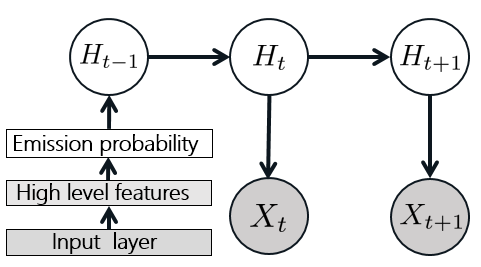
\includegraphics[width=0.3\textwidth]{images/GraphicalModel.png}\\
  \caption{Per-action model: a forward-linked chain. Inputs (skeletal features or depth image features) are first passed through Deep Neural Nets (Deep Belief Networks for skeletal modality or 3D Convolutional Neural Networks for depth modality) to extract high level features. The outputs are the emission probabilities of the hidden states.}\label{GM}
\end{figure}
\subsection{Ergodic States Hidden Markov Model}
\begin{figure}[t]
  \centering
  % Requires \usepackage{graphicx}
  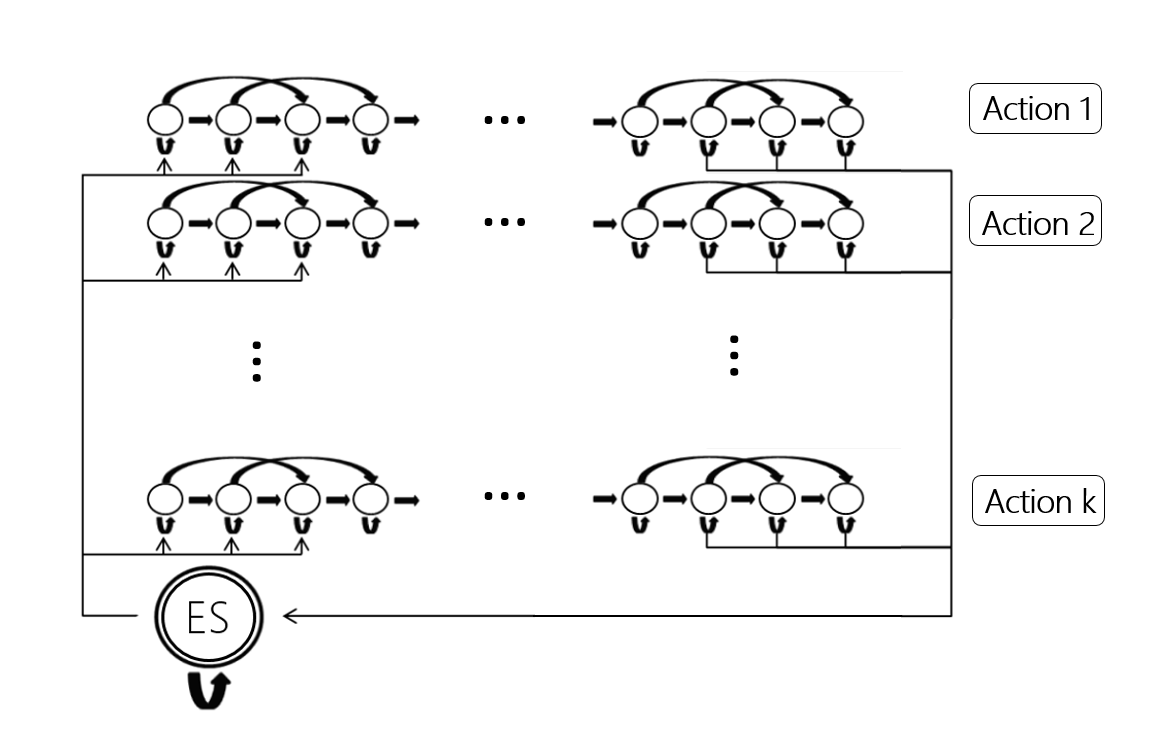
\includegraphics[width=0.48\textwidth]{images/HMM_2.png}\\
  \caption{
    State diagram of the \emph{ES-HMM} model for low-latency action segmentation and recognition. An ergodic states (ES) shows the resting position between action sequence. Each node represents a single frame and each row represents a single action model. The arrows indicate possible transitions between states.}
    \label{HMM_ES}
\end{figure}
The aforementioned framework can be easily adapted for simultaneous action segmentation and recognition by adding an ergodic states (\emph{$\mathcal{ES}$}) which resembles the silence state for speech recognition. Hence, the unobserved variable $H_t$ takes an extra finite set $\mathcal{H}=(\bigcup _{a \in \mathcal{A}} \mathcal{H}_a) \bigcup \mathcal{ES}$, where $\mathcal{ES}$ is the ergodic state as the resting position between actions and we refer the model as Ergodic States Hidden Markov Model (\emph{ES-HMM}) for simultaneously gesture segmentation and recognition.

Since our goal is to capture the variation in speed of performing gestures, we set the transitions in the following way: when being in a particular node $n$ in time $t$, moving to time $t + 1$, we can either stay in the same node (slower performance), move to node $n + 1$ (the same speed of performance), or move to node $n+2$ (faster performance). From the $\mathcal{ES}$ we can move to the first three nodes of any gesture class, and from the last three nodes of any gesture class we can move to the $\mathcal{ES}$  as shown in Fig.~\ref{HMM_ES}.

The \emph{ES-HMM} framework differs from the Firing Hidden Markov Model of~\cite{nowozin2012action} in that we strictly follow the temporal independent assumption, forbidding inter-states transverse, preconditioned that a non-repetitive sequence would maintain its unique states throughout its performing cycle.

\begin{flushleft}
\textbf{\emph{Hidden states}($\mathcal{H}_a$): } Force alignment is used to extract the hidden states, \emph{i.e.}, if a gesture token is 100 frames, the first 10 frames are assigned as hidden state $\textbf{\emph{1}}$ and the 10-20 frames are assigned as hidden state $\textbf{\emph{2}}$ and so on and so forth.

\textbf{\emph{Ergodic states($\mathcal{ES}$)}:} Neutral frames are extracted as 5 frames before or after a gesture tokens labelled by ground truth.
\end{flushleft}

The emission probability of the trained model is represented as a matrix of size $N_{\mathcal{TC}} \times N_{\mathcal{F}}$ where $N_{\mathcal{F}}$ is the number of frames in a test sequence and output target class $N_{\mathcal{TC}}=N_{\mathcal{A}} \times N_{\mathcal{H}_a}+1$ where $N_{\mathcal{A}}$ is the number of action class and $N_{\mathcal{H}_a}$ is the number of states associated to an individual action $a$ and one $\mathcal{ES}$ state (\emph{c.f.} Fig. \ref{Sample0700_comparison}: x-axis as $N_{\mathcal{F}}$ and y-axis as $N_{\mathcal{TC}} $ with $\mathcal{ES}$ as the bottom y-axis 101).


Once we have the trained model, we can use the normal online or offline smoothing, inferring the hidden marginal distributions $p(H_t | X_t)$  of every node (frame) of the test video.
Because the graph for the Hidden Markov Model is a directed tree, this problem can be solved exactly using the max-sum algorithm. The number of possible paths through the lattice grows exponentially with the length of the chain. The Viterbi algorithm searches this space of paths efficiently to find the most probable path with a computational cost that grows only linearly with the length of the chain~\cite{bishop2006pattern}.
We can infer the action presence in a new sequence by Viterbi decoding as:
 \begin{equation}
    V_{t,\mathcal{H}}= P(H_t | X_t)+\log (\max_{\mathcal{H} \in \mathcal{H}_a}( V_{t-1,\mathcal{H}}))
    \label{viterbi_GDBN}
\end{equation}
where initial state $V_{1,\mathcal{H}}=\log(P(H_1 |X_1))$.
From the inference results, we define the probability of an action $a \in \mathcal{A}$ as $p(y_t=a|x_{1:t}) =V_{T,\mathcal{H}}$.
Result of the Viterbi algorithm is a path--sequence of nodes which correspond to hidden states of gesture classes. From this path we can infer the class of the gesture (\emph{c.f.} Fig. \ref{Sample0700_comparison}).
The overall algorithm for training and testing are presented in Algorithm \ref{MMDDN_train} and \ref{MMDDN_test} .





\begin{algorithm}
\caption{Multimodal Deep Dynamic Networks -- training}\label{MMDDN_train}
\LinesNumbered
\SetAlgoLined
\SetAlgoNoEnd
\DontPrintSemicolon
\SetKwFunction{zeroes}{zeroes}
\KwData{\;
          $ \mathbf{X^1=\{ x^1_i\}_{i \in [1 \ldots t]}}$ - raw input(skeletal) feature \; \hspace{1cm} sequence.\;
          $ \mathbf{X^2=\{ x^2_i\}_{i \in [1 \ldots t]}}$ - raw input(depth) feature sequence\;
           \hspace{1cm}in the form of     $M_1 \times M_2 \times T$, where $M_1, M_2$ are\;
           \hspace{1cm}  the height and width of the input image and $T$ \;
           \hspace{1cm}  is the number of contiguous frames of the \;
           \hspace{1cm} spatio-temporal cuboid. \;
          $ \mathbf{Y=\{ y_i\}_{i \in [1 \ldots t]}}$  - frame based local label (achieved by\; \hspace{1cm} semi-supervised forced-aligment), where \;
          \hspace{1cm} $ \mathbf{y_i} \in \{ C * S + \textbf{\emph{1}} \} $ with $C$ is the number of class,\;
          \hspace{1cm} $S$ is the number of hidden states for each class, \;
          \hspace{1cm} $\textbf{\emph{1}}$ as ergodic state.
            }
\For{$m \leftarrow 1$ to $2$}{
    \SetAlgoVlined
    \eIf{$m$ is $1$}{
        Preprocessing skeletal data $ \mathbf{X^1}$ as in Eq.\ref{sk_features_1} \ref{sk_features_2} \ref{sk_features_3}.\;
        Normalizing(zero mean, unit variance per dimension) the above features and feed to to Eq.\ref{GRBMenergy}. \;
        Pre-training the networks using \emph{Contrastive Divergence}. \;
        Supervised fine-tuning the Deep Belief Networks using $ \mathbf{Y}$ by standard mini-batch \emph{SGD} backpropagation.\;
    }{
        Preprocessing the depth and RGB data $ \mathbf{X^2}$ as in \ref{3d_preproc}.\;
        Feeding the above features to Eq.\ref{ReLU}. \;
        Training the 3D Convolutional Neural Networks using $ \mathbf{Y}$.\;
    }
}
\KwResult{\;
        $\mathbf{GDBN}$ - a gaussian bernoulli visible layer Deep \;
                \hspace{1cm} Belief Network to generate the emission \;
                \hspace{1cm} probabilities for hidden markov model.\;
        $\mathbf{3DCNN}$ - a 3D Deep Convolutional Neural \;
                    \hspace{1cm}Networks to generate the emission probabilities\;
                    \hspace{1cm} for hidden markov model.\;
        $\mathbf{p(H_1)}$ - prior probability for $ \mathbf{Y}$.\;
        $ \mathbf{p(H_t | H_{t-1})}$ - transition probability for $ \mathbf{Y}$,  enforcing\;
                \hspace{1cm} the beginning and ending of a sequence can \;
                \hspace{1cm} only start from the first or the last state.
}
\end{algorithm}
%%%%%%%%%%%%%%%%%%%%%%%%%%%%%%%%%%%%%%%%%%%%%%%%%%%%%%%%%%%%%%%%%%%%%%%%%%%%%%%%%%%%%%%%%%%%%%%%%%%%%%%%%%%%%%%%
\begin{algorithm}[t]
\caption{Multimodal Deep Dynamic Networks -- testing}\label{MMDDN_test}
\LinesNumbered
\SetAlgoLined
\SetAlgoNoEnd
\DontPrintSemicolon
\SetKwFunction{zeroes}{zeroes}
\KwData{\;
         $\mathbf{X^1=\{x^1_i\}_{i \in [1 \ldots t]}}$ - raw input(skeletal) feature \; \hspace{1cm} sequence.\;
         $\mathbf{X^2=\{x^2_i\}_{i \in [1 \ldots t]}}$ - raw input(depth) feature sequence\; \hspace{1cm}in the form of $M \times M \times T$. \;
         $\mathbf{GDBN}$ - trained gaussian bernoulli visible layer  \;
                \hspace{1cm} Deep Belief Network to  generate the emission\;
                 \hspace{1cm} probabilities for hidden markov model.\;
         $\mathbf{3DCNN}$ - trained  3D Deep Convolutional Neural\;
                    \hspace{1cm} Networks to generate the emission\;
                    \hspace{1cm} probabilities for hidden markov model.\;
        $\mathbf{p(H_1)}$ - prior probability for $ \mathbf{Y}$.\;
        $ \mathbf{p(H_t | H_{t-1})}$ - transition probability for $ \mathbf{Y}.$
            }

\For{$m \leftarrow 1$ to $2$}{
    \SetAlgoVlined
    \eIf{$m$ is $1$}{
        Preprocessing and normalizing the data $ \mathbf{X^1}$  as in \ref{sk_features_1} \ref{sk_features_2} \ref{sk_features_3}.\;
        Feedforwarding network $\mathbf{GDBN}$ to generate the emission probability $\mathbf{p(X_t | H_t )}$ in Eq.\ref{HMM_GM_1}. \;
        Generating the score probability matrix $\mathbf{S^1 = p(H_{1:T},X_{1:T}).}$ \;
    }{
        Preprocessing the data $ \mathbf{X^2}$ (normalizing, median filtering the depth data).\;
        Feedforwarding $\mathbf{3DCNN}$ to generate the emission probability $\mathbf{S^2 = p(X_t | H_t )}$ in Eq.\ref{HMM_GM_1}. \;
        Generating the score probability matrix $\mathbf{S^2 =p(H_{1:T},X_{1:T}).}$ \;
    }
}
        Fusing the score matrix $\mathbf{S = \alpha * S^1 + (1-\alpha)* S^2}$. \;
        Finding the best path $\mathbf{V_{t,\mathcal{H}}}$ using $\mathbf{S}$ by Viterbi decoding as in Eq.\ref{viterbi_GDBN}. \;
\KwResult{\;
        $ \mathbf{Y=\{ y_i\}_{i \in [1 \ldots t]}}$  - frame based local label  \;
                       \hspace{1cm}  where $ \mathbf{y_i} \in \{ C * S + \textbf{\emph{1}} \} $ with $C$ is the number\;
                       \hspace{1cm}  of class, $S$ is the number of hidden states for\;
                       \hspace{1cm}  each class, $\textbf{\emph{1}}$ as ergodic state. \;
        $ \mathbf{C}$ - global label, the anchor point is chosen as the\;
                        \hspace{1cm} middle state frame.\;
}
\end{algorithm}


\section{Model Implementation}
 In all our experiments the number of states associated to an individual action $N_{\mathcal{H}_a} $ is chosen as 5 for modeling the states of an action class, therefore $N_{\mathcal{TC}}= 20 \times 5 + 1 = 101$.
\subsection{Skeleton Module}
\begin{figure}[t]
  \centering
  % Requires \usepackage{graphicx}
  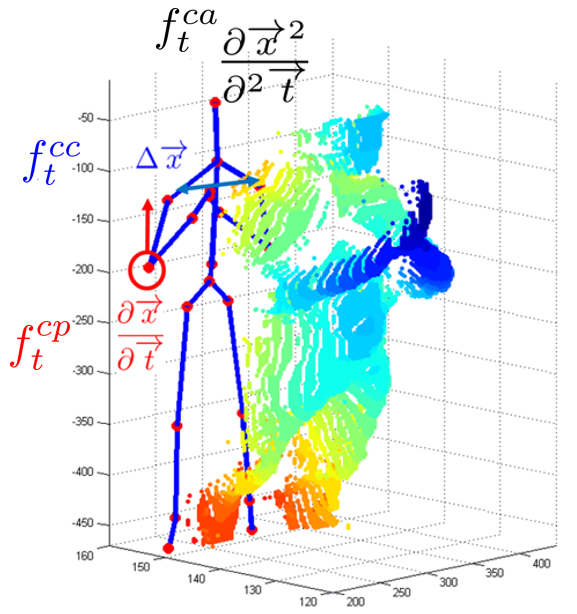
\includegraphics[width=0.3\textwidth]{images/point_cloud}\\
  \caption{
    Point cloud projection of depth image and the 3D positional features.}
    \label{point_cloud}
\end{figure}
\subsubsection{Preprocessing}
Only upper body joints are relevant to the discriminative gesture recognition tasks. Therefore, only the 11 upper body joints are considered. The 11 upper body joints used are \emph{``ElbowLeft, WristLeft, ShoulderLeft, HandLeft, ElbowRight, WristRight, ShoulderRight, HandRight, Head, Spine, HipCenter"}.


The 3D coordinates of $N$ joints of frame $c$ are given as: $X_c=\{x_1^c,x_2^c, \ldots, x_N^c\}$. 3D positional pairwise differences of joints~\cite{diwucvpr14} are deployed for observation domain $\mathcal{X}$. They capture posture features, motion features  by direction concatenation: $\mathcal{X}=[f_{cc}, f_{cp}, f_{ca}]$ as in Eq. \ref{sk_features_1} \ref{sk_features_2} \ref{sk_features_3}. Note that offset features $f_{ci}$ used in ~\cite{diwucvpr14} depend on the first frame, if the initialization fails which is a very common scenario, the feature descriptor will be generally very noisy. Hence, the offset features $f_{ci}$ are discarded and only the two more robust features $[f_{cc}, f_{cp}, f_{ca}]$ (as shown in Fig. \ref{point_cloud}) are kept:
\begin{align}
%f_{cc}&=\{x_i^c-x_j^c | i,j=1,2,\ldots,N; i\neq j \}     \label{sk_features_1}\\
%f_{cp}&=\{x^c_i-x^p_j | x^c_i \in X_c; x^p_j \in X_p \}  \label{sk_features_2}\\
%f_{cp}&=\{x^c_i-x^p_j | x^c_i \in X_c; x^p_j \in X_p \}   \label{sk_features_3}
%f_{ca}&=\{x^p_j - 2 \times x^c_i + x^c_n | x^c_i \in X_c; x^p_j \in X_p; x^c_n \in X_n   \} \label{sk_features_3} 
f_{cc}&=\{x_i^c-x_j^c | i,j=1,2,\ldots,N; i\neq j\} \label{sk_features_1}\\
f_{cp}&=\{x^c_i-x^p_i | x^c_i \in X_c; x^p_i \in X_p \} \label{sk_features_2}\\
f_{ca}&=\{x^p_i - 2 \times x^c_i + x^n_i | x^c_i \in X_c; x^p_i \in X_p; x^n_i \in X_n   \} \label{sk_features_3} 
\end{align}
with $X_i^c, X_i^p, X_i^n$ as the current, previous, next frame skeletal features.

This results in a raw dimension of  $N_{\mathcal{X}}=N_{joints} * ( \frac{ N_{joints}}{2} + N_{joints}+ N_{joints})*\mathit{3}$ where $N_{joints}$ is the number of joints used. Therefore, in the experiment with $N_{joints}=11, N_{\mathcal{X}}=891$.
Admittedly, we do not completely neglect human prior knowledge about information extraction for relevant static postures, velocity and offset overall dynamics of motion data.
Nevertheless, the aforementioned three attributes are all very crude pairwise features without any tweak into the dataset or handpicking the most relevant pairwise, triple wise, \emph{etc.} , designed features.%~\cite{chaudhry2013bio,muller2006motion,nowozin2012action,ofli2013sequence}.

A similar data driven approach has been adopted in~\cite{fothergill2012instructing} where random forest classifiers were adapted to the problem of recognizing gestures using a bundle of 35 frames. These sets of feature extraction processes resemble the \emph{Mel Frequency Cepstral Coefficients (MFCCs)} for the speech recognition community~\cite{mohamed2012acoustic}.
%\textbf{\emph{Caveat}}:
%\begin{itemize}
%\item  When extracting skeletal features, the 3D joint coordinates have not been transformed from the world coordinate system to a person centric coordinate system by placing the \emph{``HipCenter"} at the origin.
%\item  Note also that the normalization scheme by scaling the skeleton position using length of \emph{``HipCenter"} and \emph{``Spine"} didn't work well in the implementation.
%\item The third point worth noting is that some actors performed gestures using left hand as a dominant hand whereas some using right hand which worth investigating the effect of this in the future. However, those tokens are treated indiscriminately.  Hence, the feature fed into \emph{GRBM} are almost raw, un-preprocessed.
%\end{itemize}
\subsubsection{Gaussian Bernoulli Restricted Boltzmann machines}
Because input skeletal features(\emph{a.k.a.}observation domain $\mathcal{X}$) are continuous instead of binomial features, we use the Gaussian RBM (\emph{GRBM}) to model the energy term of first visible layer:
\begin{equation}
    E(v,h;\theta) =-\sum^D_{i=1} \frac{(v_i-b_i)^2}{2\sigma_i^2} -\sum^D_{i=1} \sum^F_{j=1} W_{ij}  h_j \frac{v_i}{\sigma_i}- \sum^F_{j=1}a_jh_j
\label{GRBMenergy}
\end{equation}

The conditional distributions needed for inference and generation are given by:
\begin{equation}
    P(h_{j=1}|\textbf{v})=g(\sum_i W_{ij}v_i+a_j));
\end{equation}
\begin{equation}
    P(v_{i=1}|\textbf{h})=\mathscr{N}(v_i|\mu_i,\sigma_i^2).
\end{equation}
where $\mu_i=b_i+\sigma_i^2 \sum_j W_{ij} h_j$ and $\mathscr{N}$ is normal distribution. In general, we normalize the data (mean substraction and standard deviation division) in the preprocessing phase. Hence, in practice, instead of learning $\sigma_i^2$, one would typically use a fixed, predetermined unit value $\textbf{\emph{1}}$ for $\sigma_i^2$.

For high level skeleton feature extraction, the network architectures is $[N_{\mathcal{X}},2000,2000,1000,N_{\mathcal{TC}}]$,
 where $N_{\mathcal{X}} = 891$ is the observation domain dimension; $N_{\mathcal{TC}}$ is the output target class.


\subsubsection{Deep Belief Networks Pretraining \& Training Details}
 In the training set, there are in total $400,117$ frames. During the training of \emph{DBN}, $90\%$ is used for training, $8\%$ for validation (for the purpose of early stopping ) $2\%$ is used for test evaluation.
The feed forward networks are pre-trained with a fixed recipe using stochastic gradient decent with a mini-batch size of 200 training cases. Unsupervised initializations tend to avoid local minima and increase the network�s performance stability and we have run 100 epochs for unsupervised pre-training. For Gaussian-binary RBMs, learning rate is fixed at 0.001 while for binary-binary RBMs as 0.01 (note in generally training \emph{GRBM} requires smaller learning rate). For fine-tuning, the learning rate starts at 1 with 0.99999 mini-batch scaling. Maximum number of fine-tuning epoch is 500 with early stopping strategy and during the experiments, early stopping occurs around 440 epoch.
Optimization complete with best validation score (the frame based prediction error rate) of $38.19\%$, with test performance $38.11\%$.

Though we believe further carefully choosing network architecture would lead to more competitive results, in order not to ``creeping overfitting", as algorithms over time become too adapted to the dataset, essentially memorizing all its idiosyncrasies, and losing ability to generalize~\cite{torralba2011unbiased}, we would like to treat the model as the aforementioned more generic approach.
Since a completely new approach will initially have a hard time competing against established, carefully fine-tuned methods. More fundamentally, it may be that the right way to treat dataset performance numbers is not as a competition for the top place.
This way, fundamentally new approaches will not be forced to compete for top performance right away, but will have a chance to develop and mature.
The performance of skeleton module is shown in Tab~\ref{Table_score_fusion}. 



\subsection{RGB \& Depth 3D Module}
\subsubsection{Preprocessing}\label{3d_preproc}
Working directly with raw input Kinect recorded data frames, which are $480 \times 640$ pixel images, can be computationally demanding. Deepmind technology~\cite{mnih2013playing} presented the first deep learning model to successfully learn control policies directly from high-dimensional sensory input using deep reinforcement learning.

Our first step in the preprocessing stage is cropping the highest hand and the upper body using the given joint information. We discovered that the highest hand is the most interesting. If both hands are used, they perform the same (mirrored) movement. If one hand is used, it is always the highest one. If the left hand is used, the videos are mirrored. This way, the model only needs to learn one side.

The preprocessing results in four video samples (body and hand with gray-scale and depth) of resolution 4x64x64 (4 frames of size 64x64). Furthermore,the noise in the depth maps is reduced with thresholding, background removal using the user index, and median filtering. The outcome is shown in Figure~\ref{3dcnn input}.
\begin{figure}[t]
  \centering
  % Requires \usepackage{graphicx}
  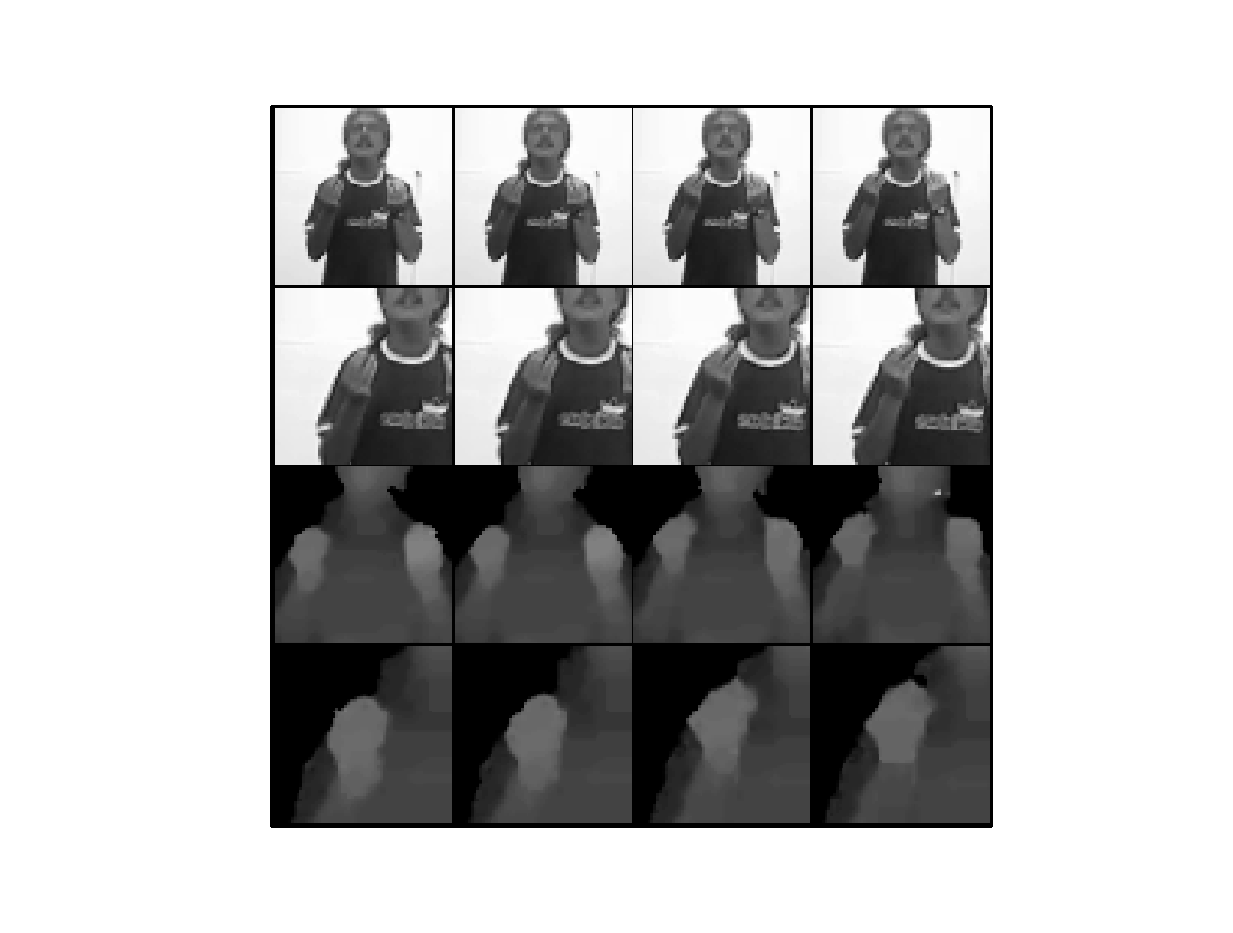
\includegraphics[width=0.5\textwidth]{images/3dcnn_filters/original.eps}\\
  \caption{
    Preprocessing steps. Inputs  from top to bottom: 1) gray-scale body input, 2) gray-scale hand input, 3) depth body input, 4) depth hand input. }
    \label{3dcnn input}
\end{figure}


\subsubsection{3DCNN Architecture}
\begin{figure*}[t]
  \centering
  % Requires \usepackage{graphicx}
  \includegraphics[width=.9\textwidth]{images/3dcnn}
  \caption{An illustration of the architecture of the 3DCNN architecture.}\label{3dcnn_architecture}
\end{figure*}

The 3D convolution is achieved by convolving a 3D kernel to the cuboid formed by stacking multiple contiguous frames together. We follow the nomenclature as in~\cite{ji20133d}.
 However, instead of using $tanh$ unit as in~\cite{ji20133d}, the Rectified Linear Units (\emph{ReLUs})~\cite{krizhevsky2012imagenet} were adopted where trainings are several times faster than their equivalents with $tanh$ units.
 Formally, the value of a unit at position $(x, y, z)$ ($z$ here corresponds the time-axis) in the $j$th feature map in the $i$th layer, denoted as $v^{xyz}_{ij}$, is given by:
\begin{equation}
v^{xyz}_{ij} =  max( 0,  ( b_{ij} + \sum_m \sum_{p=0}^{P_i - 1} \sum_{q=0}^{Q_i -1 } \sum_{r=0}^{R_i -1} w^{pqr}_{ijm} v^{(x+p)(y+q)(t+r)}_{(i-1)m} ))
\label{ReLU}
\end{equation}

The 3DCNN architecture is depicted as Fig.~\ref{3dcnn_architecture} : the 4 types ~\ref{3dcnn input} of input contextual frames are stacked as size $64\times64\times4$. The depth images are normalized with $N_{var}$ and the grayscale images are normalized with $N_{std}$ as in \ref{normalization1},\ref{normalization2} because the median of depth images is irrelevant to the gesture subclass but the grayscale images is.
\begin{align}
N_{var} &= (x -\emph{\textbf{mean}}(x)) / (\textbf{\emph{var}}(x))^{1/2}  \label{normalization1}\\
N_{std} &= x / (\textbf{\emph{var}}(x))^{1/2}
\label{normalization2}
\end{align}

The first layer contains 32 maps of $5\times5$ kernel followed by local contrast normalization (LCN) layer~\cite{jarrett2009best} and stride (2,2,2) max pooling, then the grayscale channel and depth channel are concatenated; the second convolutional layers has 64 maps of $5\times5$ kernel followed by LCN layer and stride (2,2,2) max pooling; the third convolution layer is composed of 64 maps of $4\times4$ kernel followed by stride (1,2,2) max pooling; then all convnets outputs are flattened with the body channel and hand channel concatenated into one fully connected layer of size $1024$; the output layer $N_{\mathcal{TC}}$ is of size $ 101 = 5\times20+1$ (number of hidden states for each class$\times$ number of classes plus one ergodic state).




\subsubsection{Details of Learning}
The first 650 batches are used for training and the rest 50 files for validation.
During training, dropout \cite{hinton2012improving} and is used as main approaches to reduce overfitting with Nesterov�s accelerated gradient descent (NAG) \cite{sutskever2013importance} with a fixed momentum-coefficient of 0.9 and mini-batches of size 64.
The learning rate is initialized at 0.003 with a 5\% decrease after each epoch. The weights of the CNNs are randomly initialized with a normal distribution with $\mu = 0$ and $\sigma = 0.04$.

The frame-based classification error ran for 40 epochs is $39.062$ as validation error \ref{error rate} .

\begin{figure}[t]
  \centering
  % Requires \usepackage{graphicx}
  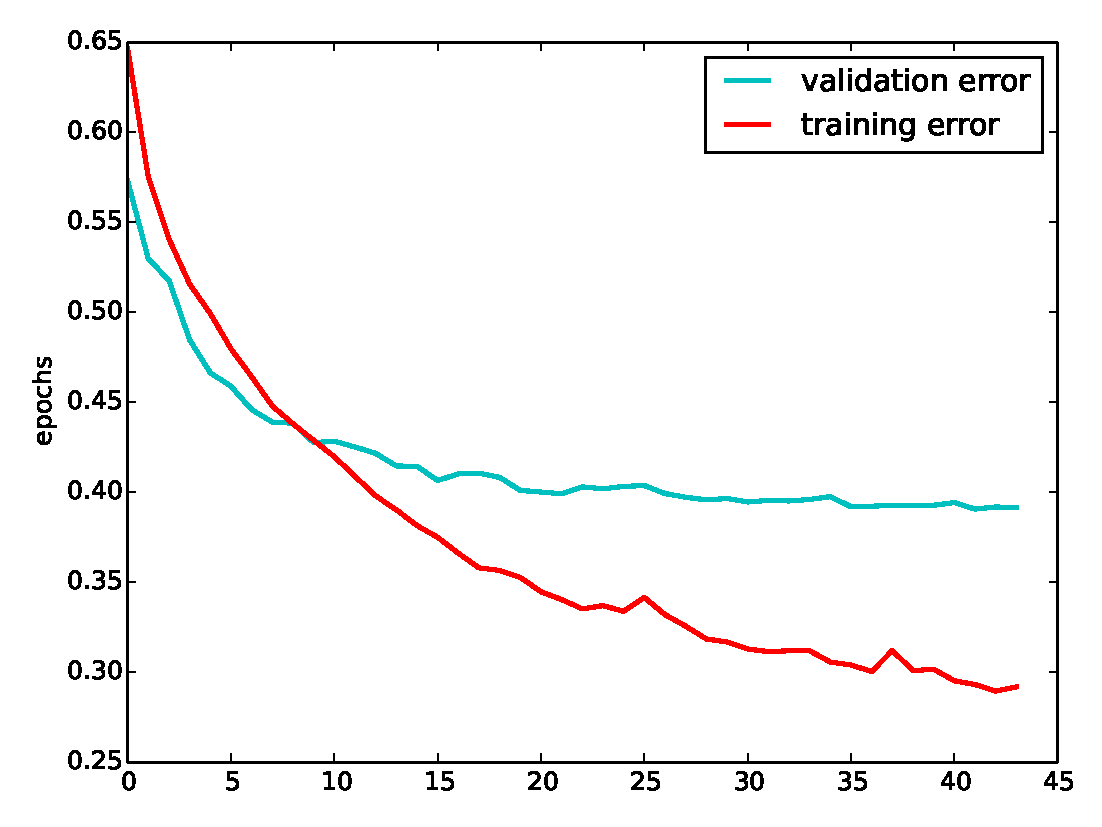
\includegraphics[width=.4\textwidth]{images/3dcnn_filters/training_error}
  \caption{The frame-based error rate for training 3DCNN.}\label{error rate}
\end{figure}

\subsubsection{Looking into the networks: visualization of filter banks}

The weight filters of the first \emph{conv1} layer are illustrated in Fig~\ref{3dcnn_filters} and it can be seen the unique characteristics from the filter kernels. For body and hand filters, both inputs are of the same size : $64\times64$. Hand inputs are smoother than the body inputs, hence the hand part filters are smoother than the body part filters. For depth and grayscale image filters: depth images generally have less edges/smoother. Hence, depth filters are smoother than the grayscale filters (though the distinctions are less obvious compared with the body vs. hand part filters).


\begin{figure}[t]
        \centering
        \begin{subfigure}[c]{.5\textwidth}
                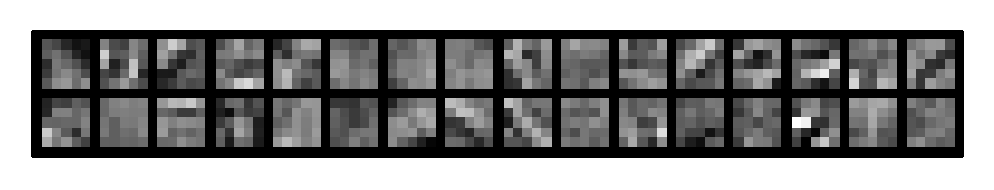
\includegraphics[width=\textwidth]{images/3dcnn_filters/gray_body_conv1_5_5}
                \caption{grayscale body part filters}
                \label{Template_Image}
        \end{subfigure}%
        ~ %add desired spacing between images, e. g. ~, \quad, \qquad, \hfill etc.
          %(or a blank line to force the subfigure onto a new line)

        \begin{subfigure}[c]{0.5\textwidth}
                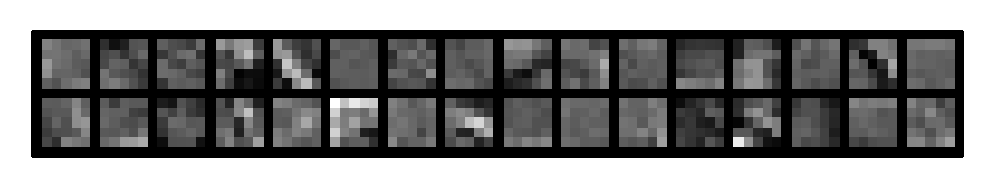
\includegraphics[width=\textwidth]{images/3dcnn_filters/depth_body_conv1_5_5}
                \caption{depth body part filters}
                \label{Test_Image}
        \end{subfigure}

        ~ %add desired spacing between images, e. g. ~, \quad, \qquad, \hfill etc.
          %(or a blank line to force the subfigure onto a new line)
        \begin{subfigure}[c]{0.5\textwidth}
                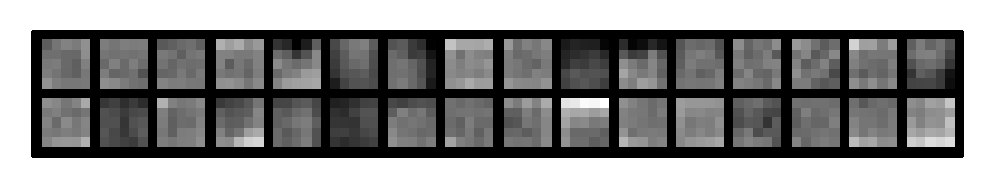
\includegraphics[width=\textwidth]{images/3dcnn_filters/gray_hand_conv1_5_5}
                \caption{grayscale hand part filters}
                \label{Template_Response}
        \end{subfigure}

        \begin{subfigure}[c]{0.5\textwidth}
        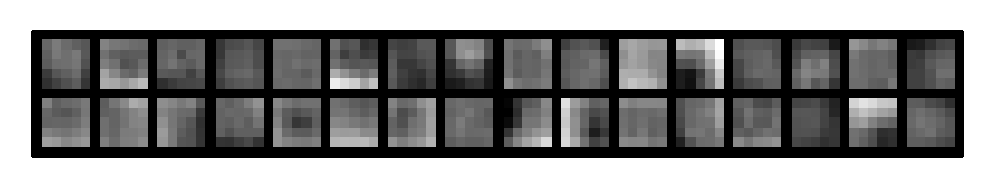
\includegraphics[width=\textwidth]{images/3dcnn_filters/depth_hand_conv1_5_5}
        \caption{depth hand part filters}
        \label{shift-resize_image}
        \end{subfigure}

        \caption{Visualization of \emph{conv1} layer for different input channels. It can be seen that the hand filters are smoother than the body part filters because hand input are smoother than the body part input.}\label{3dcnn_filters}
\end{figure}



%\begin{figure}[h]
%  \centering
%  % Requires \usepackage{graphicx}
%  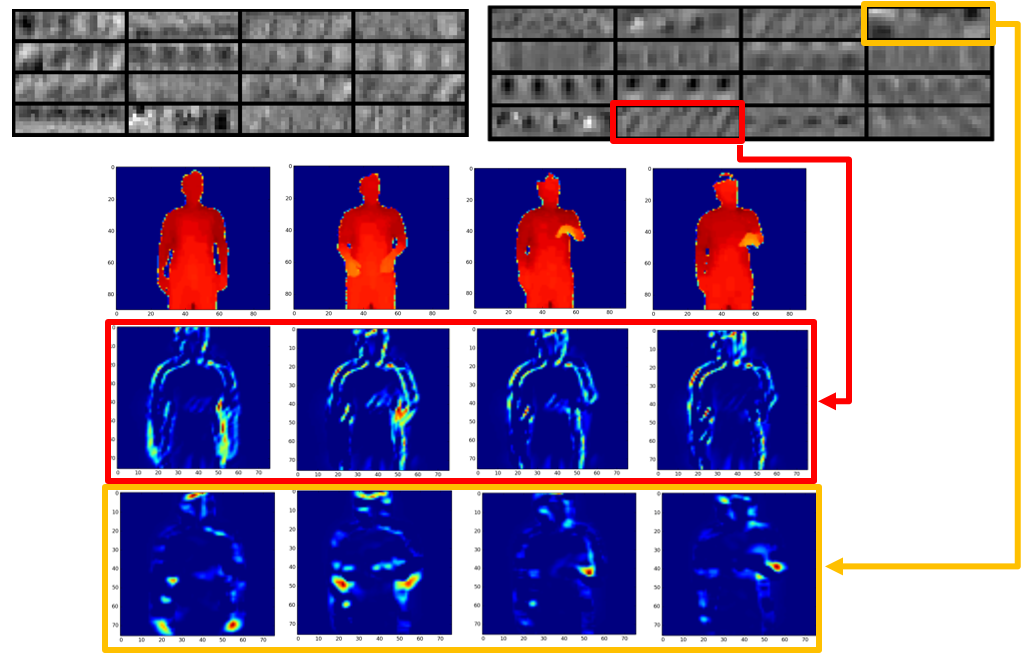
\includegraphics[width=0.5\textwidth]{images/filter_all_2}
%  \caption{{\footnotesize
%  Top left: the \emph{conv1} weights of the 3DCNN learnt with uncropped input; top right: the \emph{conv1} weights of the 3DCNN learnt with cropped input. It can be seen that filters/weights of the cropped input trained networks are smoother. Bottom: visualization of sample frames after \emph{conv1} layer (Sample0654, 264-296 frames, sampled every 8 frames). It can be seen that the filters of the first convolutional layer are able to learn both shape pattern(red bounding box) and motion(yellow bounding box). Also note that the high response maps correspond to the most informative part of the body, even though during the training process, all local patches are learned indiscriminately regardless of its location.}
%  }\label{conv1_vis}
%\end{figure}


%\begin{algorithm}[t]
%\caption{Normalization scheme 1: template matching}\label{normalization_scheme_1}
%\LinesNumbered
%\SetAlgoLined
%\SetAlgoNoEnd
%\DontPrintSemicolon
%\SetKwFunction{zeroes}{zeroes}
%\KwData{\;
%          $ \mathbf{T}$ - exemplary template with original scale of size $320 \times 320$,   \;
%           \hspace{0.5cm}   (Sample0003 is chosen as the exemplary template, shown in \ref{Template_Image}). \;
%          $ \mathbf{R_{depth}}$  - reference depth, fixed to $\textbf{\emph{1941}}$ (acquired from the above \;
%             \hspace{0.5cm} exemplary template  $ \mathbf{T}$). \;
%          $ \mathbf{\hat{T}}$ - test image, as shown in \ref{Test_Image}.\;
%          $ \mathbf{M}$ - user foreground segmented mask. \;
%            }
%        Apply a $5 \times 5$ aperture median filter to test depth frame $\mathbf{\hat{T}}$ as in~\cite{wu2012one} to reduce the salt and pepper noise. \;
%        Multiply test depth frame $\mathbf{\hat{T}}$ with the user segmented mask $ \mathbf{M}$: $\mathbf{\hat{T} = \hat{T} \times M}$. \;
%        Template matching test image $\mathbf{\hat{T}}$ with $ \mathbf{T}$ using normalized cross-correlation~\cite{lewis1995fast}, the response score $\mathbf{R}$  is shown in \ref{Template_Response}. \;
%        Shift the image according to the maximum response $\mathbf{R}$ to its centre applying affine transformation~\cite{opencv_library}. \;
%        Scale the image according to reference depth $ \mathbf{R_{depth}}$ and the median depth of a bounding box in the centre of the image with $25 \times 25$ size as shown as the green boundingp box in \ref{shift-resize_image}. \;
%        Resize the image from $320 \times 320$ to $90 \times 90$. \;
%
%
%\KwResult{\;
%        $ \mathbf{\tilde{T}}$ - Resize-normalized image shown in the yellow bounding box of \ref{shift-resize_image}.\;
%}
%\end{algorithm}
%\begin{algorithm}
%\caption{Normalization scheme 2: skeleton normalization}\label{normalization_scheme_2}
%\LinesNumbered
%\SetAlgoLined
%\SetAlgoNoEnd
%\DontPrintSemicolon
%\SetKwFunction{zeroes}{zeroes}
%\KwData{\;
%          $ \mathbf{S_{spine}}$ - Skeleton Spine joints pixel coordinates. \;
%          $ \mathbf{S_{shoulder}}$ - Skeleton Shoulder joints pixel coordinates. \;
%          $ \mathbf{\hat{T}}$ - test image.\;
%          $ \mathbf{M}$ - user foreground segmented mask. \;
%          $ \mathbf{R_{length}}$  - reference length of shoulder to spine, fixed to $\textbf{\emph{100}}$ (1 meter). \;
%            }
%        Apply a $5 \times 5$ aperture median filter to test depth frame $\mathbf{\hat{T}}$. \;
%        Multiply test depth frame $\mathbf{\hat{T}}$ with the user segmented mask $ \mathbf{M}$. \;
%        Shift the image according to the centroid of Spine joint $ \mathbf{S_{spine}}$.\;
%        Scale the image according to the $\mathbf{R_{length}}  / (\mathbf{S_{spine}} - \mathbf{S_{shoulder}})$. \;
%
%\KwResult{\;
%        $ \mathbf{\tilde{T}}$ - Resize the shifted-scaledp image to $90 \times 90$ .\;
%}
%\end{algorithm}
%\begin{figure}[t]
%        \centering
%        \begin{subfigure}[c]{0.2\textwidth}
%                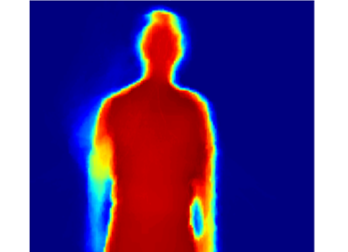
\includegraphics[width=\textwidth]{images/template3}
%                \caption{{\scriptsize template image}}
%                \label{Template_Image}
%        \end{subfigure}%
%        ~ %add desired spacing between images, e. g. ~, \quad, \qquad, \hfill etc.
%          %(or a blank line to force the subfigure onto a new line)
%        \begin{subfigure}[c]{0.2\textwidth}
%                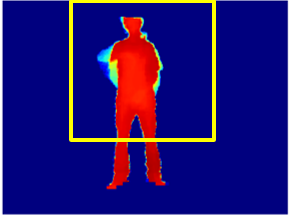
\includegraphics[width=\textwidth]{images/test1}
%                \caption{{\scriptsize test image}}
%                \label{Test_Image}
%        \end{subfigure}
%        ~ %add desired spacing between images, e. g. ~, \quad, \qquad, \hfill etc.
%          %(or a blank line to force the subfigure onto a new line)
%        \begin{subfigure}[c]{0.2\textwidth}
%                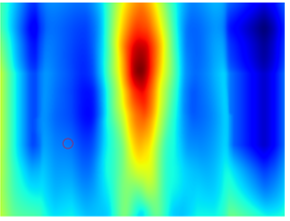
\includegraphics[width=\textwidth]{images/test3}
%                \caption{{\scriptsize template response}}
%                \label{Template_Response}
%        \end{subfigure}
%        \begin{subfigure}[c]{0.2\textwidth}
%        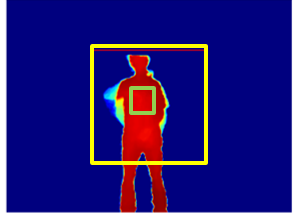
\includegraphics[width=\textwidth]{images/test2}
%        \caption{{\scriptsize shift-resize image}}
%        \label{shift-resize_image}
%        \end{subfigure}
%        \caption{{\footnotesize Illustration of normalization scheme 1: template matching.}}\label{Normalization scheme 1: template matching}
%\end{figure}

\section{Related Works}
This paper served as the progressive works of ~\cite{wu2014deep} and ~\cite{lio2014deep}.

To highlight the difference between our previous works of ~\cite{wu2014deep}, ~\cite{lio2014deep}.

~\cite{neverova2014multi} present a multi-scale and multi-modal deep networks for gesture detection and localization. Key to their technique is a training strategy that exploits i) careful initialization of initialization of individual modalities and ii) gradual fusion of modalities from strongest to weakest cross-modality structure. One major difference between our proposed method and theirs is the treatment of time element. In ~\cite{neverova2014multi}, the proposed networks requires fixed length inputs and in order to cope with various action speed, a multiscale network is required which potentially increase the time for training and testing. 

Some of the top winning methods ~\cite{neverova2014multi}~\cite{Monnier2014multi}~\cite{Chang2014multi}~\cite{Peng2014multi} in this challenges requires a set of complicated handcrafted features

1)wudi 3dcnn multiple networks average works better And it can be seen that larger net (Net2) will generally perform better than smaller net (Net1), averaging multi-column nets almost will certainly further improve the performance~\cite{ciresan2012multi}. Hence, in the following experiments, only the multi-column averaging results are reported.

2) first ranks skeleton is extremely complicated


\section{Experiments and Analysis}
\subsection{Chalearn LAP Dataset \& Evaluation Metrics}
This dataset\footnote{\href{http://gesture.chalearn.org/homewebsourcereferrals}{http://gesture.chalearn.org/homewebsourcereferrals}}  is on ``multiple instance, user independent learning and continuous gesture spotting"~\cite{ICMI} of gestures. And in the 3 track, there are more than 14,000 gestures are drawn from a vocabulary of 20 Italian cultural/anthropological sign gesture categories with 700 sample sequences for training and validation and 240 sample sequences for testing.

For input sequences, there are three modalities, \emph{i.e.} skeleton, RGB and depth (with user segmentation) provided. In the following experiments, the first 650 sample sequences are used for training, 50 for validation and the rest 240 for testing where each sequence contains around 20 gestures with some noisy non-meaningful vocabulary tokens.

The evaluation criteria for this track is the \emph{Jaccard} index (overlap) on a frame-to-frame basis.
\begin{equation}
J(A, B) = \frac{A \bigcap B}{A \bigcup B}
\end{equation}

\subsection{Post-Processing}
The predicted token less than 20 frames are discarded as noisy tokens. Note that there are many noisy gesture tokens predicted by viterbi decoding. One way to sift through the noisy tokens is to discard the token path log probability small than certain threshold. However, because the metric of this challenge: \emph{Jaccard index} strongly penalizes false negatives, experiments show that it's better to have more false positives than to miss true positives. Effective ways to detect false positives should be an interesting aspect of future works.


\subsection{Score Fusion}
\begin{figure}[t]
  \centering
  % Requires \usepackage{graphicx}
  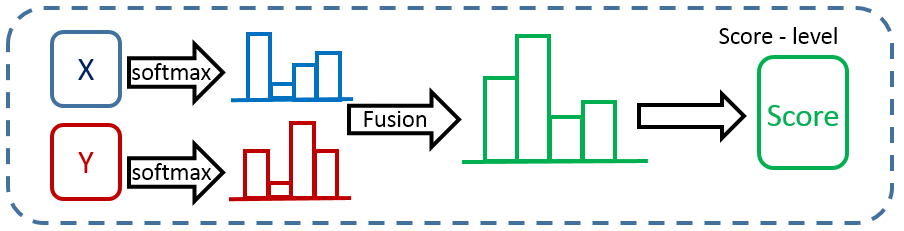
\includegraphics[width=0.45\textwidth]{images/fusion}
  \caption{
 Illustration of descriptor fusion.
  }\label{fusion}
\end{figure}

To fuse the dual model prediction, the strategy shown as Fig \ref{fusion} is adopted. The complementary properties of both modules can be seen from the Viterbi path decoding plot in Fig \ref{Sample0700_comparison} :

\begin{equation}
 \mathbf{S} = \alpha*\mathbf{S^1} + (1-\alpha) * \mathbf{S^2}
\end{equation}
where $\mathbf{S^1}$ and $\mathbf{S^2}$ are the score probability matrix as in Algo. \ref{MMDDN_test}, corresponding to the skeletal input and depth \& RGB input, and $\alpha$ is the coefficient controls the score balance obtained by cross validation. Interesting, the best $\alpha$ is around $0.5$ which means the almost equal importance of the two modules.


Note that the skeleton module generally performs better than the depth module, one reason could be that the skeleton joints learnt from~\cite{shotton2011real} lie in success of utilizing huge and highly varied training data: from both realistic and synthetic depth images, a total number of 1 million images were used to train the deep randomized decision forest classifier in order to avoid overfitting. Hence skeleton data are more robust.



 \begin{table}[t]
   \centering
        \begin{tabular}{|l||*{2}{c|}}\hline
            \backslashbox{Module}{Evaluation Set}
            &\makebox[8em]{Validation}&\makebox[6em]{Test}
            \\\hline\hline
            {\small Skeleton--DBDN }            &  0.78266    & 0.76900 \\\hline
            {\small Depth \& RGB --3DCNN }      &  0.75163    & 0.71678 \\\hline
            {\small Score Fusion }              &  0.81744    & 0.80910 \\\hline\hline
        \end{tabular}

    \caption{
    Comparison of results in terms of Jaccard index between different network structures and various modules.
          }
          \label{Table_score_fusion}
\end{table}


\begin{figure*}[t]
        \centering
        \begin{subfigure}[c]{.8\textwidth}
                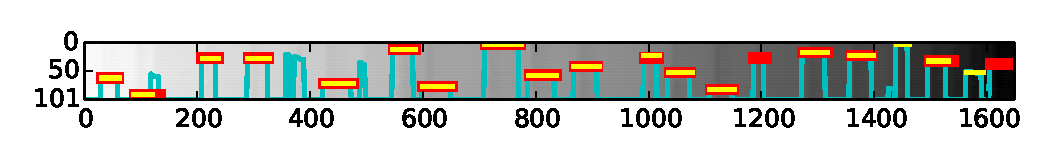
\includegraphics[width=\textwidth]{images/path/Sample0700_sk}
                \caption{Sample 700 skeleton input path.}
                \label{Sample0700_sk}
        \end{subfigure}%
        ~ %add desired spacing between images, e. g. ~, \quad, \qquad, \hfill etc.
          %(or a blank line to force the subfigure onto a new line)

        \begin{subfigure}[c]{0.8\textwidth}
                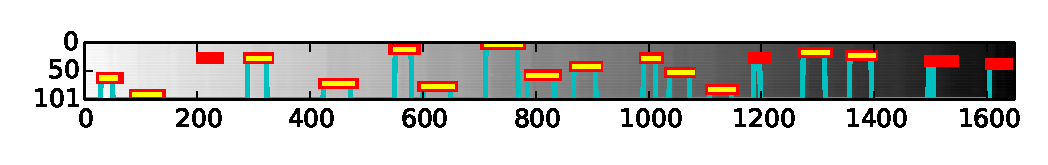
\includegraphics[width=\textwidth]{images/path/Sample0700_cnn}
                \caption{Sample 700 depth and RGB input path.}
                \label{Sample0700_cnn}
        \end{subfigure}

        ~ %add desired spacing between images, e. g. ~, \quad, \qquad, \hfill etc.
          %(or a blank line to force the subfigure onto a new line)
        \begin{subfigure}[c]{0.8\textwidth}
                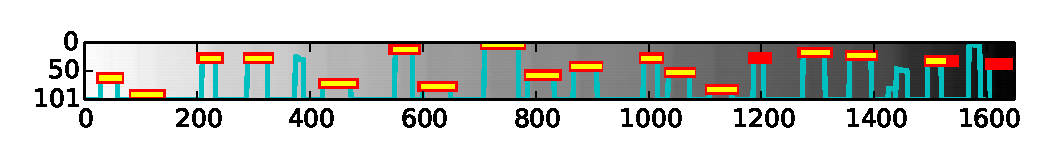
\includegraphics[width=\textwidth]{images/path/Sample0700_combined}
                \caption{Sample 700 combined input path.}
                \label{Sample0700_combined}
        \end{subfigure}

  \caption{Viterbi decoding of two modules and their fusion result of sample sequence 700. Top to bottom: skeleton, depth \& RGB, score fusion with x-axis representing the time and y-axis representing the hidden states of all the classes with the ergodic state at the bottom. Red lines are the ground truth label, cyan lines are the viterbi shortest path and yellow lines are the predicted label. There are some complementary information of the two modules and generally skeletal module outperforms the depth module. The fusion of the two could exploit the uncertainty, \emph{e.g.}, around frame 200 skeleton can help with the false negative prediction given by CNN module and around frame 1450, CNN module can help suppress the false positive prediction given by skeleton module.
  }\label{Sample0700_comparison}
\end{figure*}

\subsection{Computational complexity}
Though learning the Deep Neural Networks using stochastic gradient descent is tediously lengthy, once the model finishes training, with a low inference cost, our framework can perform real-time video sequence labeling.
Specifically, a single feed forward neural network incurs trivial computational time ($\mathcal{O}(T)$) and is fast because it requires only matrix products and convolution operations. The complexity of Viterbi algorithm is $\mathcal{O} (T* |S|^2)$ with number of frames $T$ and state number $S$.

\section{Conclusion and Discussion}

Hand-engineered, task-specific features are often less adaptive and time-consuming to design. This difficulty is more pronounced with multimodal data as the features have to relate multiple data sources.
In this paper, we presented a novel Deep Dynamic Neural Networks(DDNN) framework that utilizes Deep Belief Networks and 3D Convolutional Neural Networks for learning contextual frame-level representations and modeling emission probabilities for Markov Field.
 The heterogeneous inputs from skeletal joints and depth images require different feature learning methods and the late fusion scheme is adopted at the score level. The experimental results on bi-modal time series data show that the multimodal DDNN framework can learn a good model of the joint space of multiple sensory inputs, and is consistently as good as/better than the unimodal input, opening the door for exploring the complementary representation among multimodal inputs. It also suggests that learning features directly from data is a very important research direction and with more and more data and flops-free  computational power, the learning-based methods are not only more generalizable to many domains, but also are powerful in combining with other well-studied probabilistic graphical models for modeling and reasoning dynamic sequences.
Future works include learning the share representation amongst the heterogeneous inputs at the penultimate layer and backpropagating the gradient in the share space in a unified representation.


\appendices
% you can choose not to have a title for an appendix
% if you want by leaving the argument blank
\section{Details of the Code}
The python project for  can be found at: \\
{\verb+https://github.com/stevenwudi/chalearn2014_wudi_lio+}


% use section* for acknowledgment
\ifCLASSOPTIONcompsoc
  % The Computer Society usually uses the plural form
  \section*{Acknowledgments}
\else
  % regular IEEE prefers the singular form
  \section*{Acknowledgment}
\fi

The authors would like to thank...



\bibliographystyle{IEEEtran}
\bibliography{tPAMI2015}




% biography section
%
% If you have an EPS/PDF photo (graphicx package needed) extra braces are
% needed around the contents of the optional argument to biography to prevent
% the LaTeX parser from getting confused when it sees the complicated
% \includegraphics command within an optional argument. (You could create
% your own custom macro containing the \includegraphics command to make things
% simpler here.)
%\begin{IEEEbiography}[{\includegraphics[width=1in,height=1.25in,clip,keepaspectratio]{mshell}}]{Michael Shell}
% or if you just want to reserve a space for a photo:


\begin{IEEEbiography}{Di Wu}
Biography text here.
\end{IEEEbiography}

% if you will not have a photo at all:
\begin{IEEEbiography}{Lionel Pigou}
Biography text here.
\end{IEEEbiography}

\begin{IEEEbiography}{Ling Shao}
Biography text here.
\end{IEEEbiography}

\begin{IEEEbiography}{Lio's Mentor}
Biography text here.
\end{IEEEbiography}
% insert where needed to balance the two columns on the last page with
% biographies
%\newpage


% You can push biographies down or up by placing
% a \vfill before or after them. The appropriate
% use of \vfill depends on what kind of text is
% on the last page and whether or not the columns
% are being equalized.

%\vfill

% Can be used to pull up biographies so that the bottom of the last one
% is flush with the other column.
%\enlargethispage{-5in}



% that's all folks
\end{document}


